\documentclass{beamer}
 
\usepackage[utf8]{inputenc}
\usepackage[fontset=ubuntu]{ctex}
\usetheme{Madrid}
\usepackage{graphicx}
\usepackage{amsmath}
 
%Information to be included in the title page
\title{MATH5905}
\subtitle{Hypothesis Testing \& Order Statistics}
\author{Chenxuan Rong}
\date{2018-10-7}
 
 
\begin{document}
 
\frame{\titlepage}
 
\begin{frame}
    \frametitle{Table of Contents}
\tableofcontents
\end{frame}

\section{hypothesis testing}
    \begin{frame}
        \frametitle{Basic Concepts in hypothesis testing}
        

        \begin{itemize}
            \item 
            type I error: P(reject $H_0$ | $H_0$ is correct) = level of test
            \item
            type II error: P(accept $H_0$ | $H_1$ is correct) = 1 - power of test
        \end{itemize}
        
        \begin{block}{minimise type I error}
        \begin{itemize}
            \item increase accept region
            \item increase sample size
        \end{itemize}
        \end{block}
        

        \begin{itemize}
            \item
            \textbf{null hypothesis} is often an initial claim that is based on previous analyses or specialised knowledge
            \item
            \textbf{alternative hypothesis} is what you might believe to be true or hope to prove true.
            \item
            simple hypothesis: $H_0:\theta = \theta_0$\\
            simple alternative: $H_1: \theta = \theta_1$
        \end{itemize}
    \end{frame}
    
    \begin{frame}{Basic Concepts in hypothesis testing}
        \begin{itemize}
            \item test: $\phi(x)=P(reject\ H_0|X=x)$
            \item $\alpha$(size, level of significance): probability of rejection $H_0$ when it is correct
            \item $\beta$(power): probability of rejection $H_0$ when $H_1$ is correct
        \end{itemize}
        
        \begin{alertblock}{Note}
        minimising level and maximising power simultaneously is \textbf{not possible}!
        \end{alertblock}
        
        Approaches we take:
        \begin{itemize}
            \item fix certain value $\alpha$ that is not allowed to be exceed for type I error
            \item find the one with the smallest type II error(= highest possible power)
        \end{itemize}
    \end{frame}
    
    \begin{frame}{Motivation - What we are trying to do?}
        \begin{itemize}
            \item 在满足$\alpha$的限制条件下,找到有最大power的test\\
            \item \href{https://onlinecourses.science.psu.edu/stat414/node/305/}{如何把test statistic转化成sample mean?}
        \end{itemize}
    \end{frame}
    
    \begin{frame}{Different type of Hypothesis illustration}
        \begin{figure}
        \centering
        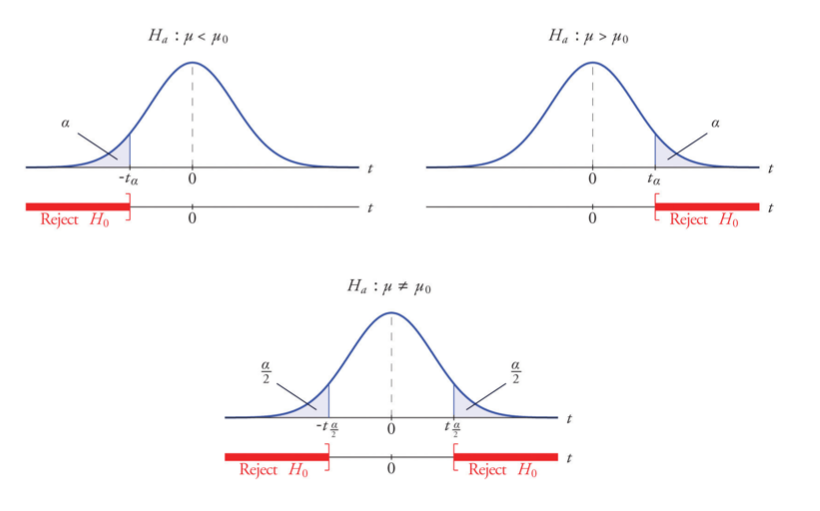
\includegraphics[width=10cm]{cr}
        \end{figure}
    \end{frame}
    
    \begin{frame}{Neyman-Pearson Lemma}
        \[
        \phi(x)^*= 
        \begin{cases}
            1,&\text{if } x \in S = {x:L(x,\theta_1)/L(x,\theta_0) > C},\\
            \gamma, &\text{if } x \in S = {x:L(x,\theta_1)/L(x,\theta_0) = C},\\
            0,&\text{if } x \in S = {x:L(x,\theta_1)/L(x,\theta_0) < C}
        \end{cases}
        \]
        with $E_{\theta_0}\phi^*=\alpha$, $\gamma=\frac{\alpha-P_{\theta_0}(S)}{P_{\theta_0}(R)}$
        \begin{block}{注意}
        这条定理适用于simple hypothesis的情况,如果是compound hypothesis的情况,找most powerful test需要用uniformly most-powerful test的方法
        \end{block}
    \end{frame}
    
    \begin{frame}{Monotone Likelihood Ratio}
        \begin{block}{Definition}
            $\frac{L(x,\theta^{''})}{L(x,\theta^{'})}$ is a non-decreasing function of $T(x)=T(x_1,x_2,...x_n)$\\
            \textbf{Note:}\\
            For one-parameter exponential family, if $c(\theta)$ is monotone increasing, this family has MLR in $T(x)=\Sigma_{i=1}^{n}d(X_i)$
        \end{block}
        
        \begin{exampleblock}{Examples}
            Tutorial3 - Q1
        \end{exampleblock}
    \end{frame}
    
    \begin{frame}{Blackwell \& Girshick Theorem}
    Suppose $X \sim L(x,\theta)$ and the family is with MLR in T(X). Then for testing $H_0:\theta \leq \theta_0$ versus $H_1:\theta > \theta_0$, the $\alpha-test\ \phi^*$ with the structure:
        \[
        \phi(x)^*= 
        \begin{cases}
            1,&\text{if } T(X) > k,\\
            \gamma, &\text{if } T(X) = k,\\
            0,&\text{if } T(X) < k
        \end{cases}
        \]
    (k is the upper $\alpha.100\%$ point) has an increasing power function $E_{\theta}\phi^*$
        \begin{alertblock}{Note}
            该定理适用的情况是$H_0:\theta \leq \theta_0$ versus $H_1: \theta > \theta_0$
        \end{alertblock}
        \begin{block}{Difficulties}
            What does "exhaust the level" mean?\\
            How to calculate k?
        \end{block}
    \end{frame}
    
    \begin{frame}{Plot Power Function}
    解题步骤:
        \begin{itemize}
            \item 找出T(X)
            \item 证明MLR在T(X)上单调(monotone)
            \item 根据BG定理构建test(看清假设的形式!)
            \item 通过$E_{\theta_0}\phi^*=\alpha$求K
            \item 作图Power function
        \end{itemize}
    \end{frame}
    
    \begin{frame}{Plot Power Function}
        \begin{exampleblock}{Example 6.6.3 - Uniform}
            Assume that $X=(x_1,x_2...,x_n)$ are i.i.d from
            \[
                f(x,\theta)= 
                \begin{cases}
                    \frac{2x}{\theta^2}, 0<x<\theta\\
                    0,&\text{else }
                \end{cases}
            \]
            Construct a UMP $\alpha-test$ of $H_0:\theta \leq \theta_0$ versus $H_1:\theta > \theta_0$
        \end{exampleblock}
    \end{frame}

    \begin{frame}{Plot Power Function}
        \begin{exampleblock}{Example 6.6.3 - Discrete case}
        n=25, i.i.d observations from Bernoulli($\theta$), with $\alpha=0.01$ chosen for level of significance. Construct the UMP $\alpha-test$ of $H_0:\theta \leq 0.15$ versus $H_1:\theta > 0.15$
        \end{exampleblock}
        
        \begin{block}{Interpretation}
            What does the constructed test mean?
        \end{block}
    \end{frame}
    
    \begin{frame}{Other test methods}
        If no UMP test exists, what else methods could we try?
        \begin{itemize}
            \item Unbiased MPU $\alpha-tests$
            \item Locally most powerful tests
            \item Likelihood ratio tests
            \item Score test, Wald test
        \end{itemize}
    \end{frame}
        


\section{Order Statistics}
    \begin{frame}{Order Statistics}
        Recall Order statistics we've met so far:\\
        \begin{itemize}
            \item $X_{(1)}, X_{(n)}$ in uniform distribution
        \end{itemize}
        
        Why we care about order statistics?
        \begin{itemize}
            \item $X_{(n)}$ is of interest in studying floods,earthquakes
            \item $X_{(1)}$ is used for estimating strength of a chain
            \item sample median is a measure of population central tendency
            \item $(X_{(n)}+X_{(1)})/2$ is a measure of central tendency
        \end{itemize}
    \end{frame}
    
    \begin{frame}{Order Statistics - Important Theorems}
        \begin{block}{Theorem 7.3 - Find $X_{(r)}$ }
        \end{block}
        \begin{block}{Theorem 7.4 - Find joint distribution of two order statistics}
        \end{block}
        \begin{exampleblock}{Tutorial 4 - 7}
        \end{exampleblock}
    \end{frame}
    
    \begin{frame}{Multinomial distribution}
        binomial distribution的扩展形式\\
        掷硬币变成了掷骰子
    \end{frame}
    

\section{Assignment two}
    \begin{frame}{Assignment Two - Asymptotic \& Delta method}
    \begin{exampleblock}{Tutorial2 - 22}
        $f(x,\theta)=\theta x^{\theta-1}I_{(0,1)}(x), where\ \theta > 0$\\
        \begin{itemize}
            \item MLE of $\tau(\theta)=\frac{\theta}{1+\theta}$
            \item asymptotic distribution of MLE of $\tau(\theta)$ in a)
            \item Is C.R bound attainable?
        \end{itemize}
    \end{exampleblock}
    \end{frame}
    
    \begin{frame}{Assignment Two - Order Statistics}
        \begin{alertblock}{Notes on mathStatica}
            This is not a free software! GO TO MATH LAB!!\\
        \end{alertblock}
        
        \begin{block}{Some Knowledge}
            \href{http://www.mathstatica.com/software/buy.html}{mathStatica Official Site}
            mathStatica 是MATHEMATICA的付费扩展包,MATHEMATICA可以申请学生账户,但是mathStatica需要额外购买.
        \end{block}
        
    \end{frame}

\section{Exam Review Tips}
    \begin{frame}{Exam Review Tips}
        \begin{itemize}
            \item Decision Theory
            \item Sufficient Statistics, MLE, Fisher Information
            \item C.R.Bound, UMVUE, BlackWell-Rao Theorem(**)
            \item asymptotic MLE, delta method
            \item hypothesis testing, simple, compound
            \item order statistics
            \item higher order asymptotic, saddle point approximation
        \end{itemize}
    \end{frame}
    
    \begin{frame}{Contact}
        \begin{figure}
        \centering
        
\includegraphics[width=5cm]{wechat}
        \end{figure}
    \end{frame}
 
\end{document}
